\documentclass[a4paper,twocolumn]{svjour3} 

%opening
\usepackage{times}
\usepackage{enumitem}
\usepackage{graphics}
\graphicspath{{Users/wafajohal/Dropbox/WRITING/MonThese/Figures/}{Users/wafajohal/Dropbox/WRITING/MonThese/Figures/illustrate/}{Users/Users/wafajohal/Dropbox/WRITING/MonThese/Figures/plots/}}
\usepackage{hyperref}
\usepackage{graphicx}  
\usepackage{subfigure} 

\begin{document}
\title{Behavioural Styles for Child-Robot Interaction%\thanks{Grants or other notes
%about the article that should go on the front page should be
%placed here. General acknowledgments should be placed at the end of the article.}
}
\subtitle{Do you have a subtitle?\\ If so, write it here}

%\titlerunning{Short form of title}        % if too long for running head

\author{Wafa Johal         \and
        Gaelle Calvary \and %etc.
        Sylvie Pesty
}

%\authorrunning{Short form of author list} % if too long for running head

\institute{Wafa Johal \at
              first address \\
              Tel.: +123-45-678910\\
              Fax: +123-45-678910\\
              \email{fauthor@example.com}           %  \\
%             \emph{Present address:} of F. Author  %  if needed
           \and
           S. Author \at
              second address
}

\date{Received: date / Accepted: date}
% The correct dates will be entered by the editor
\maketitle
\begin{abstract}
	In this paper we present the concept of behavioural style as a tool for personalisation of robot's behaviour in specific roles. 
	We propose a study for which we have employed various kind of metrics to evaluate the perception and the influence of a robot's behavioural style on children. 
	This within subjects experiment took place in a smart apartment equipped with cameras, microphones and Kinect sensor. 16 children from 7 to 11 participated to the experiment.
	In the experiment the robot would either have an authoritative attitude or a permissive attitude. 
	We measured the influence of this attitude via various medium:
	interviews of children, questionnaires, task performances, parents observation and confrontation, and postural analysis. 
	We show that postural analysis gave the best measure to predict the style of the robot from the child's point of view.
	These results illustrate recent tendencies in HRI to go away from self-assessment measures with young children.
\keywords{First keyword \and Second keyword \and More}	
\end{abstract}

%*****************************************************************************************************
\section{Introduction}
\label{sec:introduction}
%paragraph1 : general prgagraph about context 
As technology develops, there is a tendency of the multiplication of the numerical platforms in home-environments. 
The new dynamic of the Internet-Of-Things and connected objects have accelerated this phenomenon. 
Computer devices, tablet or cellphone users haven't yet established a social relationship with them. 
Creating a social relationship with the numerical devices could help increase trust and quality of life of individuals.
Where the users used to see these platforms as tools, they should now be able to exploit these artificial entities and create a social relationship that is trustable, controllable and credible. 
To this end, this user-tool relationship should evolve into a user-companion relationship, in which the user can count on his companion to care, help and entertain him.

Human-human communication is a large detailed field of study. 
Some signals sent between human interlocutors are subconscious while still having been processed by their cognition.
Subconsciously, humans emit social signals that shows their intentions and their goals.
These abilities are parts of what is called the social intelligence.
Several research fields, from human-computer interaction, affective computing, social signal processing, human-robot interaction, human activity recognition etc. are now working on enabling new technologies with social intelligence in order to make them more user-friendly and acceptable.
Researchers in HRI~\cite{Tapus2007,Dautenhahn2007} have also noted that robots need not only to be competent in the task but also socially intelligent.

%traditionally
Researchers in Human-Robot Interaction (HRI) have agreed that acceptability in home environments will come only via sociability\footnote{\textit{\textbf{Sociability} is the ability to perceive, understand and express social cues of communication in a human-understandable way.
It is also the ability to create and maintain social relationships; the ability to learn and develop social competencies }\cite{Dautenhahn2007}.} of the robots.


%our vision
The underlying assumption of this work is that the social personalisation of the companion's robot behaviour improves the acceptability of the users.
The interest in the personalisation of companion robots comes from the assumption that users want a more socially intelligent robot while keeping a certain controllability of their home assistant.
It is also assumed that social robots should display comprehensive behaviours for the user - in its decision and expressions.
For this, its reasoning processes should be made explicit to the user providing a level of understanding. 
Customisation of the behaviours on the other hand can improve the user's feedback as well as the controllability of his companion robot.
The perspective taken in this thesis is to propose a way for the user to chose the manner their companion robot would behave. 
This aims to contribute in both acceptability of the companion and to make the relationship and social bounding easier with the companion. 
In particular, the goal for this thesis is to investigate how the personalisation of the social robot's behaviour in context based on \textit{style} can be designed and evaluated in a realistic context and can contribute to \textit{social adaptability} of the companion robot's behaviour.

The challenge of the social adaptability of a robot's behaviour can be approached from different perspectives. 
The design of companion robots requires an understanding and a model of the \textit{plasticity} as well as reasoning and developing communicating vector of this adaptation. 
Our work takes concepts from several disciplines, aiming to benefit from various approaches of plasticity.
As the research went along, this work used notions from socio-psychology, cognitive sciences, artificial intelligence and affective reasoning, human-machine interaction, computer sciences and human-robot interaction.

From a more technical point of view, the variations in the ways social roles that a social robot  has to play can be seen as styles applied to a predefined script.
The notion of style and social role are important in this thesis: the robot plays a social role with a particular style in order to fit  the social expectations of the user better.
A social role is understood as a set of abilities, goals and beliefs of the robot and the style as a way of performing the social role.

%could ...

%research questions
\paragraph{research questions}
\begin{itemize}[noitemsep,nolistsep]
	\item Why should companion robots have styles ? (Section \ref{sec:soa_styles} )
	\item What distinguishes our approach from existing approaches for personalisation? (Section \ref{sec:soa_styles})
	\item Given the physical constraints of the robots (e.g., velocity limits, variation in mechanical degrees of freedom), how can this personalisation be carried out?(Chapter \ref{cha:stylemode})
	\item Can styles (parental) expressed by robots be recognized by parents ? (Chapter \ref{cha:evalonline})
	\item What is the influence of styles on the children's behaviours? (Chapter \ref{cha:stylebotxp})
	\item How can we measure the attitude changing in an interaction with a social robot? (Section \ref{sec:soa_nv})
	\end{itemize}

%paragraph 2 others, .... last sentence but pb

%paragraph 3 : In this paper we propose ...
contrary to prior work we propse a role specific way to customize nv behaviour of robots called behavioural style
we then evaluate the expressibility of these styles on two different plateform 
we then introduce a way to measure the attitude of the user
we compare attitudes of user according to behavioural style
we show that styles have an effect on the user
we also present resulst from experimental analysis indicating that 
findings from ... test indicate  statistically significant differences un 

additionally

finally we posited that even 
we conducted a follow up experiment to test this hypothesis

in section ... we discuss examples that motivate our work and place it in the context of other related work
Section 5 introduces

Section 7 presents 

We also discuss the applicability of the proposed metric of ... to ...
Finally, we describe an additional experiment designed to assess the benefit of ... in section 8.

We conclude with recommendations for the direction of future research in Section 9.

In this paper, we describe a user experiment aiming to investigate the influence of behavioural styles displayed by a humanoid robot on the perception and the attitude of a child in interaction with this robot. 
The experiment was conducted in the smart apartment Domus\footnote{Domus is an experimental platform composed especially with a domotic apartment \url{http://domus.liglab.fr/}} at the LIG Laboratory, equipped with camera sensors, microphones and other sensors and connected objects. 


%*****************************************************************************************************

\section{Related Literature/Work}
%need for acceptabilty
Robots have mainly served in the industry as their primary utility since their usage came about.
With development in technology, robots now in our daily lives are taking up roles of assistants or entertainers. 
Because of these new contexts and the new users that come with it (who are necessarily neither experts, nor programmers) robots need to be able to interact in an intuitive way with them. 
This implies that the modern day robot has to be able to perceive it's environment and to act accordingly in a humanly acceptable and welcoming manner. 
We can imagine how robots will be useful to humans in the future, but how they will be accepted in our social lives is still a maturing domain for research.


%Context social adaptability
In order to accommodate the user, many research projects have attempted to enable the robot to display social behaviours.
The adaptation to the user is also called \textbf{personalisation}.
This section gives a review of some works on personalisation in HRI.
The customisation of the robot's appearance will not be reviewed because it is out of the scope of our research eventhought 3D printed robots such as Poppy\footnote{Poppy is an open source 3D printed robot created within the Flowers research team at INRIA Bordeaux\url{https://www.poppy-project.org/technologies/}} make appearance customisation now possible.  

In Human-Computer Interaction, two kinds of personalisation systems are distinguished \cite{Fischer2001,Oppermann1997}, the ones that automatically and dynamically change according to the user, also called \textbf{user adaptive systems}, and the ones that can be changed by the user himself, also called \textbf{user adaptable systems}. 

The term personalisation is also used in other types of research projects in which robots are given a social presence - a name, a story, a past, for example. 
We won't consider these works in this classification as we believe that a better term to qualify these works would be personification and not personalisation. 


The main difference between the two types of personalisation - \textbf{adaptive} and \textbf{adaptable} - is the control on the adaptation process. 
In the adaptive systems, the changes in the systems to adapt itself are seamless to the user's view, whereas, in adaptable systems, the user is the actor of the changes. 

Another dimension of the analysis of personalisation is the nature of the changes in the system. 
The robot can either adapt to the users social characteristics (such as emotional tendency, mood, personality) and preferences (i.e. human values) or to the users abilities (i.e. performance in a specific task, vocabulary to age, school grade).
\begin{figure}[h]
	\centering
	%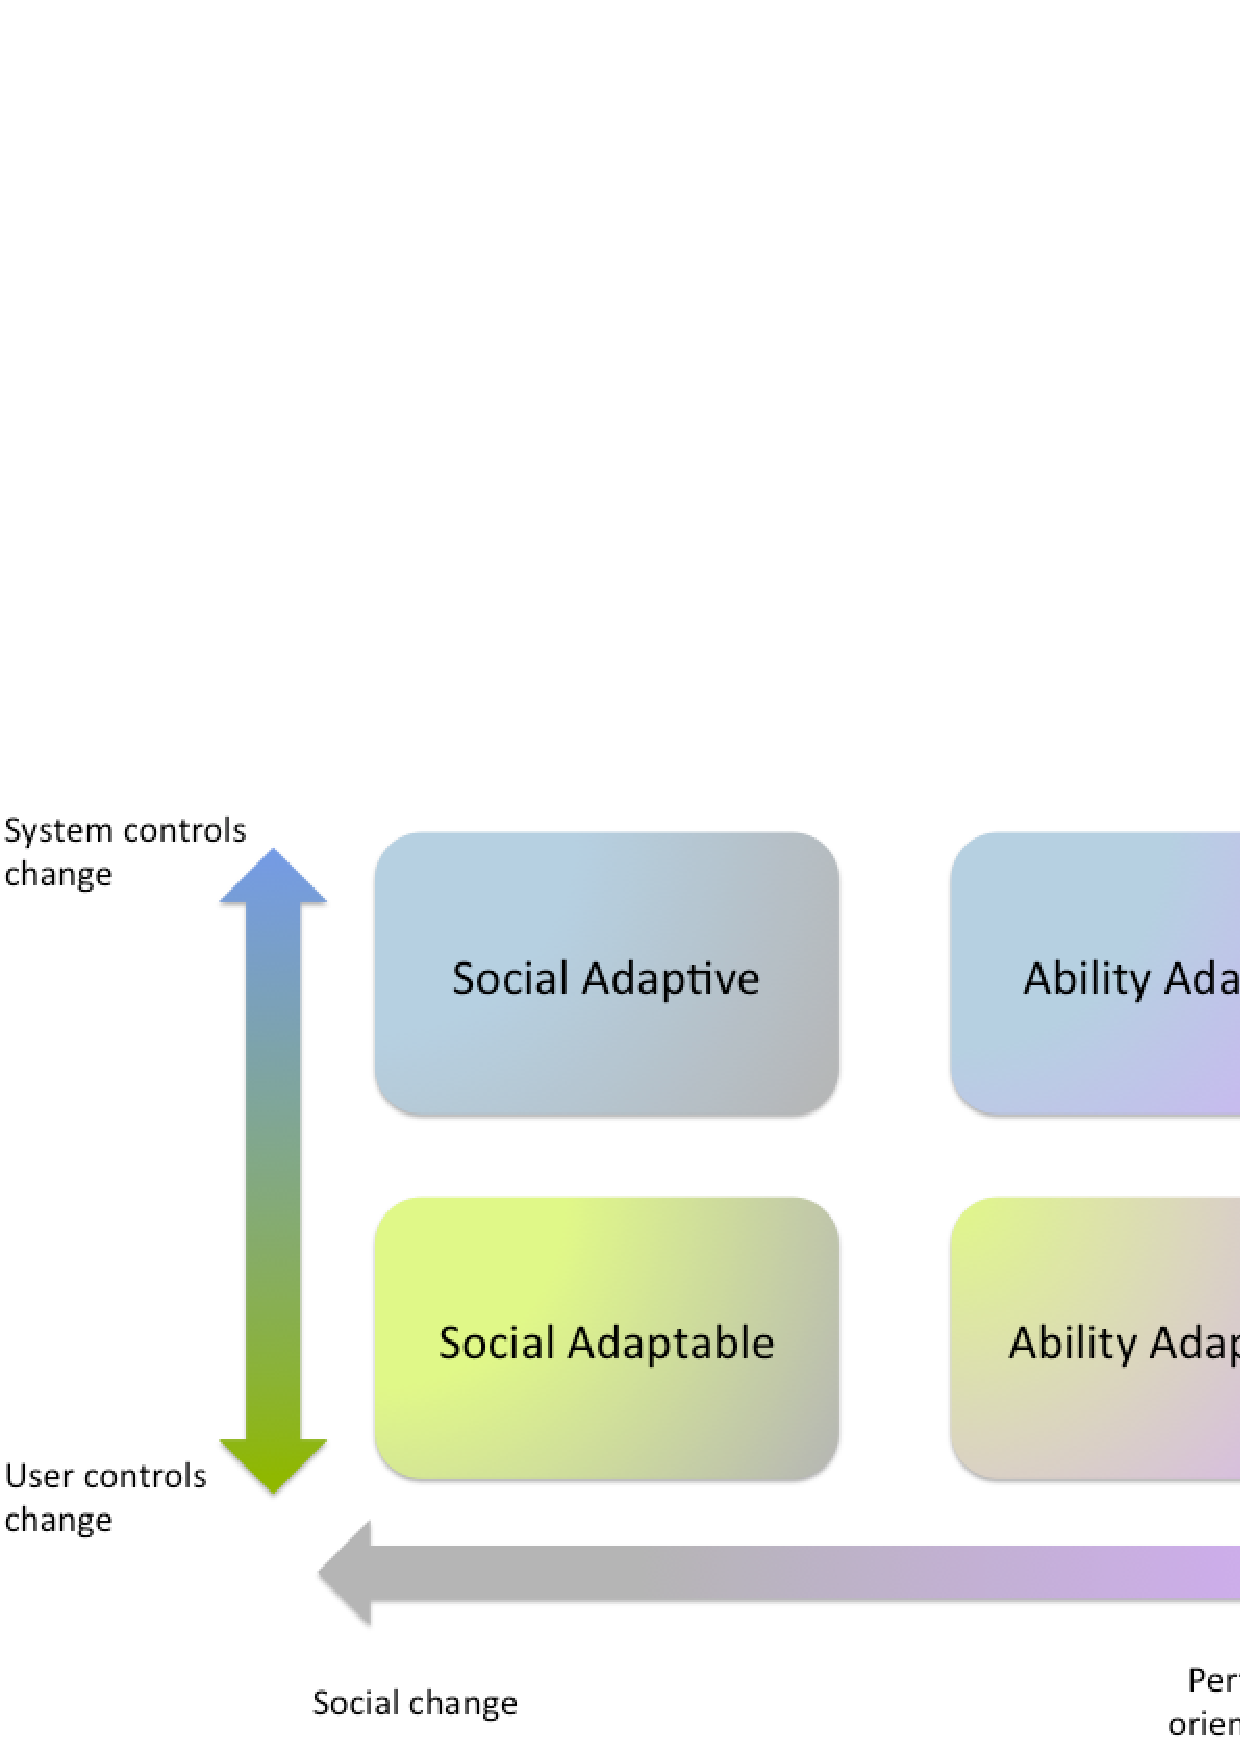
\includegraphics[width=0.9\linewidth]{personalisation}
	\caption{Categories of Personalisation in HRI}
	\label{fig:personalisation}
\end{figure}
We propose to classify personalisation systems in HRI on two dimensions as illustrated in the figure~\ref{fig:personalisation}: according to the control of the adaptation (system vs user) and the nature of the adaptation (social vs ability/task performance).

\begin{itemize}[noitemsep,nolistsep]
	\item \textbf{socially adaptive}: the system adapts itself by detecting and inferring the social preferences of the user by collecting data.
	\item \textbf{socially adaptable}: the user defines his preferences explicitly to the system. 
	\item \textbf{ability adaptive}: the systems adapt itself by learning from interactions and inferring the difficulty of the task according to the user's performances.
	\item \textbf{ability adaptable}: the users sets the difficulty by choosing the levels himself.
\end{itemize}
These different types can be combined.
For instance a teacher robot could first ask user's input to set his social preferences (cultural language sets as French for instance) and then update the user model according to performances, which would be a form of ability-adaptive and social-adaptable personalisation.
In the following part, we will present examples of works on personalisation in HRI. 

\subsection{Personalized systems in HRI}
There have been various works on personalisation in HRI. 
Individual differences are often observed in user studies in HRI. 
Personalisation can be a tool to adapt to the user's own ability and to his social preferences.
Personalisation plays a role for long-term relationship credibility, social competences and persuasion. 

\cite{Lee2012} proposed a method in which authors combined several forms of personalisation in a long-term study. 
In this study, authors used personification, adaptive and adaptable personalisation tools and concluded that personalisation improved engagement, cooperation and relationship between the participants and the robot and saw personalisation has a promising area of research in HRI. 
This study showed that personalisation was beneficial for HRI but they do not provide a framework or profiles of users. 

From the results of the study of \cite{Jones2013} within the LIREC project on teachers perspective to have a robotic tutor to assist them, personalisation turned out to be a very important requirement. 
Other research projects have highlighted this need for personalisation - the SERA\footnote{SERA: \url{http://cordis.europa.eu/project/rcn/89259_en.html}} project for instance, keen for personalisation, user or task tailoring. 
Some research works have shown that personalisation can improve the user's engagement in the task (\cite{Corrigan2013}) and the robot's competencies as perceived  by the user \cite{Fasola2012a}.


In \cite{Francois2007a}, authors proposed a \textbf{socially adaptive} robot that adapts its behaviour to the user's interaction styles. Authors collect data during the interaction and infer an interaction style. 
These works highlighted one of the difficulties in adaptive systems which being the collection of less noisy and more relevant data and the delay required for optimum socially adaptation. 
\cite{Francois2009a} improved this delay in further research but this method is still limited by the time of interaction (the more interaction, the better adaptation). 
Some other works \cite{Castro-Gonzalez2011} on learning user's preferences in term of interaction styles showed that it to be possible using Reinforcement Learning but also concluded that it would require long interactions with a larger pool of participants to determine the correct \textbf{socially adaptive} behaviour for the robot. 

Personalisation has proved in previous research to be quite effective in terms of improving acceptability and the trust of a robot. 
By showing personalised behaviour, users see the robot as more socially competent.
\cite{Kuhnlenz2013} have focused on socially adaptive robot, showing that by adapting to the mood and emotions of the user, the robot was found to be more helpful.

Personalisation has also been found to be determinant in persuasion processes. 
\cite{Fogg} claims that adapted social cues can significantly improve the persuasive impact of a computer system and that tailoring the user experience improves credibility of the system. 
This is also supported by the study of Fasola et al. \cite{Fasola2012} showing how personalisation can improve intrinsic motivation of the user. 
Some works on proxemics\footnote{Proxemics are a subcategory of non-verbal communication signals that deal with body space and posture. Hall defines four concentric space around a person the closer begin the Intimate space, around it would be, the personal space (for friend and family) the social space and then the public space \cite{hall1966}. Some modality of communication and senses were associated to these spaces.} \cite{Syrdal2007} in human-robot interaction show that there exist individual differences in term of preferred proxemics when interacting with a human. 
These non-verbal cues of communication are worth being taken into account by the robot in order to show social competence. 


Based on works on the "Theory of Companions" \cite{Kramer2011}, we choose to model companion behaviours within the social roles and to work on personalisation as a function of context. 
Section~\ref{sec:stylemode} offers a style model for socially adaptable robots' behaviours.
Hence, variability is not only the roles that the robot is expected to have, but also the way the robot will play these roles.

\subsection{Personality in HRI}
Personality is widely researched in psychology and social sciences. It is often used to characterise individual differences in terms of communication and decision making. 
There exist in HRI some systems that aim to personalise the behaviour of the robot to the user by giving the robot a personality. 
These works are social adaptation but can be either adaptable or adaptive systems. 

\cite{Revelle2009} defined \textbf{personality} as a "coherent patterning of affect, behaviour, cognition, and desires (goals) over time and space". 
Research in robots with personality is an ongoing problematic that would aim to give consistency to the companion's behaviours.
For companionship and long-term relationship, consistency is particularly important regarding the credibility and the perceived social competence of the companion. 

Some works have shown that people tend to attribute social presence and sometimes personalities to computer or interactive devices such as robots \cite{Woods2006,Meerbeek2009}. 
Often works on personality have based their work on the Five Factor Model (FFM) (also called OCEAN or Big Five) that describes personality under five dimensional traits : Openness to experience, Conscientiousness, Extraversion, Agreeableness and Neurotiscism. 


In terms of the user's adaptation of the robot personality, there has not been so far any consensus in the HRI community. 
Indeed, some studies have shown that there was a similarity attraction (an extroverted user prefers an extroverted companion robot) \cite{Isbister2000} and some others have found complementarity attraction (an extroverted user prefers an introverted companion robot \cite{Lee2006,Tapus2008}). 
\cite{Belpaeme2012a} concluded in no significant influence of extrovert and introvert personality trait in child-robot interaction.

However \cite{Joosse2013a} contested the complementary and similarity attraction theories for attribution to the user by showing that the appropriate personality is more related to the task context. 
Hence a situated personality is perceived to be more adapted and more expected by users. 
\cite{Tay2014} also recommend designing social robots within the social role framework. 
In line with this research, as Section~\ref{sec:stylemode} will show that behavioural \textbf{styles} might be seen as consistent personalised behaviour in context and hence provide consistency within a social role. 
One of our contribution is to offer a new profile-based way to make the companion robot's behaviour adaptable in an intelligible way for the user within specific social contexts. 

According to the survey of \cite{Mahani2009}, controllability, learnability and adaptability of the robot are important for user acceptability. 
Automatic social personalisation - \textbf{socially adaptive system} - have the drawback of necessitating to collect data in order to make the personalisation possible. 
Hence they are dynamic and will build on as the user interacts with the system. 
This poses questions on memory and privacy when dealing with personal data collected by a system. 

Since users often praise controllability as one of the most import criteria for acceptability, the presented approach in this thesis will follow a framework allowing \textbf{socially adaptable} behaviours by the robot.
We propose to use \textbf{styles} as tools for adaptability of the companion's behaviour within the role it has to play.

%generation or modification of motion
\subsection{Motion Generation and Modification}
BML, 
ACE, DESIRE

These systems were dedicated to programmers. 
We aim to provide a social understanding of the modified behaviiour and hence to allow the user to pick a style.

\subsection{A Quick Overview of styles in Other Domain}
\label{sec:soa_styles}
The concept of \textit{style} is widely used, and before going further it is important to define the term. 
In this section, we present different definitions of  styles found in  different fields.
In general,  styles refer to variations or ways  \textit{in doing something }, or even in \textit{appearances}.
In this review, we consider the first sense of style as a\textit{ manner or a way of doing something that would be recognisable}.
Some research domains related to ours dealing with style are reviewed in the following paragraphs: in psychology, computer sciences, computer animation and  human-robot interaction. 

\paragraph{In Psychology}:\textit{Styles} describe different ways to behave in a particular context. 
Some \textit{styles} are associated to specific social roles: management styles, teaching styles, learning styles, parenting styles. 
And there are some others such as cognitive styles that aim to classify wider preferences.
We also use the term non-role-specific styles to qualify Cognitive Styles, in opposition to role-specific styles such as  Learning, Teaching, Leadership and Parenting styles that are related to specific social roles. 
We chose as an example Parenting Styles.

Parenting Styles have been studied in socio-psychology. 
The most well-known model is Baurmind's parenting styles (\cite{baumrind1991influence}).
Maccoby and Martin updated and arranged  the parenting styles on two axis (from \cite{Darling1993}). 
The figure~\ref{fig:fpareting_style} shows these four parenting styles placed on the \textit{ dominance} and \textit{responsiveness} axes.
\begin{figure}[h]
	\centering
	%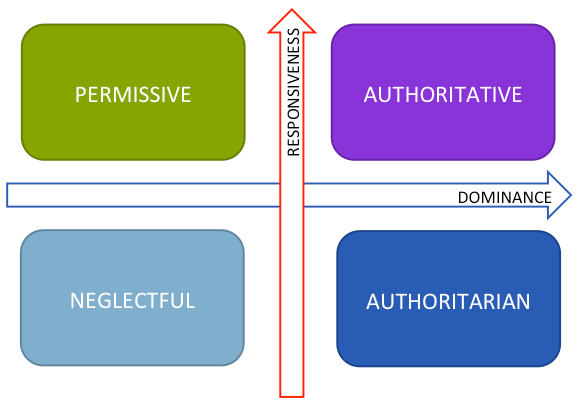
\includegraphics[width=0.7\linewidth]{../Figures/illustrate/fpareting_style}
	\caption{Parenting Styles according to two dimensions}
	\label{fig:fpareting_style}
\end{figure}


Theories of Personality aim to characterise affective and motivational invariants in the attitudes of individuals.
According to \cite{Huteau}, behaviours of individuals are characterised both by their plasticity and their consistency.
Behaviours are sensitive to situational and social contexts. 
However, there exists a singularity of behaviour in a particular situation.

To summarise the different styles that were reviewed in psychology, styles characterise intra-individual consistency in context (in the same context people tend to adopt the same style) and inter-individual differences in context (in the same context, people act differently). 
One can notice two perspectives in the way psychologists treat styles. 
It is either seen as a reflection of personality, as preferred ways. 
Or, it is seen as a strategy, a method that would suit the context in a better way. 

The link between personality and style \cite{Sternberg1997,Hayes} can be justified by the fact that styles express a preference and a continuum in the same context which can also be the expression of personality.
Some researchers in psychology even use the term Identity Styles to qualify the different kinds of personalities \cite{Berzonsky2011}.

However, unlike personalities, styles do not characterise across context consistency since the palette of styles varies according to the role played by the individual.
The review of the literature insists on context and role-specificity of styles. 
People can adopt a style in a role, even if it is not in line with their personality. 
One can be shy in his/her everyday life, while showing  self-confidence and dominance traits in a work environment .
In the same line, there are some works in psycho-therapy aiming to change ones' behaviour by using role-playing activities and letting the individual adopt the best style in the context \cite{Mehrabian1971}. 

The magnitude of these correlations confirms that personality and style are related but also suggests that when playing a social role one can suppress his/her personal preference to adopt a more suited style. 

We choose to argue for a separation of these concepts in order to let the user choose the strategy of their companion in its roles. 
Indeed, personality traits will be displayed in the behaviour of the companion when it is self-centred (for instance, when speaking about it preferences, it mood, it hobbies) but when playing a social role, one can consider that the behaviour displayed is mainly context-centred (the task, and the way the task should be performed matter more). 
We propose the figure ~\ref{fig:personality-style} to illustrate this distinction between style and personality in the expressed behaviour. 
This distinction is in line with \cite{Huteau}, who says that behaviours are characterised by consistency (referring to self-consistency and to personality) and plasticity (referring to styles and context adaptation).
Besides, apart from the cognitive styles, other styles in psychology are anchored to social roles.


As the companion robot should fulfil social roles.
Style framework  will make social behaviour design more reusable and easier to configure by the user. 
Hence, the role will be the basis on which styles can be designed to depict variations of the execution of the same role. 


\paragraph{In Animation}
Traditionally animators used key-framing techniques defining each pose of the animation and then using some interpolation technique to go from one frame(pose) to another. 
This technique is know to be expressive but less realistic than physically-based technique in which a physical model of the character drives the animation.

In order to give more expressibility to physically-based techniques, recent research in animation has been focusing in designing styles of motion. 
These styles use motion parameters in order to provide a \textbf{flexible} and \textbf{reusable} way to give expressiveness to simple motions.

In \cite{Liu2005}, authors used styles as a physically-based representation of character motion. 
In particular, this representation includes preferences of using some muscles more than others.
By combining it to other parameters they define large range of motion styles.
This style representation is said to be flexible, allowing animators to use the same style for different tasks defined independently. However, in this work, style descriptions still include an abstracted representation of the actor's anatomy.

In other works \cite{shapiro2006style}, the aim was to enable the animator to transfer a style form one motion to another to retain the same expressiveness as the original motion.
Authors show how a\textit{ clumsy style} component can be extracted form a clumsily walked motion and ported to a running motion. 
The authors also show how styles can be used for interactive analysis and editing tools for animators.

\cite{Noot2004} proposed the GESTYLE language to define variation in gestures for Embodied Conversational Agents (ECA). 
This language is written in the XML format and describes gestures by their meaning allowing the usage of different gestures to express the same thing.
GESTYLE proposes style dictionaries that specify different styles containing profession, culture, age, gender or personality informations.
In that sense, styles defined in GESTYLE are mainly self-centred (personality) rather than role/context-centred (see our distinction between style and personality - Figure~\ref{fig:personality-style}). 
The separation between content (action) and style in not clear within GESTYLE as styles are associated to specific behaviour repertoires.
For \cite{Noot2004}, behavioural style influences the choice of certain gestures, which can limit the reusability and the flexibility of the styles.
This work is interesting in the choice of annotating language and meaningful utterance with nonverbal modalities to display variations in the usage of gestures.

\cite{Rajagopal2012} continued this work and proposed to clone users' motion style into an ECA using gestures edited via BML(Behavior Markup Language).
This work showed that the used parameters to describe the \textit{wrist gesture style} were very efficient as 75\% of participants were able to discriminate a person (among two people) seen via the animation of their avatar.
Other works have been proposed to generate stylistic behaviours by first collecting data and then extracting features that characterised moods, attitude and personality \cite{Kang2013a,Czy2009}. 
These works gave good simulation results but were not making a clear distinction between the style repertoire and the context. 
It is probable that new data collection recorded in new contexts will lead to different style parameters.

Recent works in HRI showed how \textbf{behavioural styles} \cite{Ligthart2013,VandenBrule2014} could affect the trust that a user gives to the robot in accomplishing its task. 
This work highlights the importance of non-verbal cues of communications in the perceived performance of the robot in a particular context. 


To conclude, styles in HRI have been researched only recently. 
Some research teams have focussed on interaction styles - the way users interact with the robot, and some more recent works start to explore \textbf{behavioural styles} as a way to personalise the robot's behaviour within a task. 
Most of the works aiming to build stylistic expressive gestures were based on machine learning techniques that were extracted from the context of action. 
For instance, one would register several people doing the same gesture while recording their motions using a Mocap system.
They would then extract the inter-individual specificity of the motion.
This can produce a lot of motion styles, but they can be semantically weak.
However, works in psychology suggests that styles have a strong link to the social role in which they are expressed. 
This thesis contributes by proposing a meaningful way to express style based on social roles and style descriptions in psychology.

\section{Style model}
Several expressibility parameters exist to characterise motion. 
We used some of these parameters to filter pre-designed motions and to generate \textit{styled} motion.

Our definition of \emph{Behavioural Styles} is in line with psychological role-dependent styles, and hence takes into account the role played by the robot.
Before giving details in the model and the generation process of \textit{styled} behaviour, let us clarify the properties of our behavioural styles:
\begin{itemize}[noitemsep]
	\item described by a list of parameters
	\item expressed in non-verbal cues of communication
	\item associated to a meaningful concept in psychology in order to be understandable by the end-user
\end{itemize}


\subsection{Design Approach}
In this section, the different modules involved in the style model are described. 
Then, we detail on the implementation and give some examples of style sheet and application on the Nao  and Reeti robots are given.


As presented previously, the \textbf{Plasticity} perspective is taken in order to render an adaptable companion robot.
Styles characterise the plasticity of the behaviour (variability in the same context) as opposed to the personality that characterises the behaviour consistency (consistency across contexts).
Our approach aims to apply plasticity concepts to HRI as it was applied in HCI. 

As described by \cite{Coutaz2012}, the context of use modelling, in which different styles can be applied is presented by the presence of three concepts :
\begin{itemize}[noitemsep,nolistsep]
\item the role: which corresponds to the social role for the companion robot.
\item the entities involved: corresponding to the number of robots involved and their competencies (role they can play).
\item the situational inter-relation: the listener, the speaker (one can also specify here the spatial position of the agents).
\end{itemize}


On top of the roles, behavioural styles, as previously mentioned, will affect the non-verbal expressibility within the role.

The notion of style is in this model: a set of behavioural changes that can be applied to any motion of a role repertoire and that leads to a meaningful interpretation of the way the motion is executed. 
A style filter is used to generate behaviours according to the role and to the user's preferences. 
Only a few styles have been implemented for our experiments but the solution that we propose can be extended.
The aim is that users could choose the styles from a catalogue and set the one they prefer, providing hence the adaptability of the companion within the social role. 

As for CSS, the aim in the style framework for design of social behaviour for robots is to make them \textbf{reusable }and \textbf{flexible}.
We intent then to show that styles can be applied to various gestures and pre-defined behaviour but also used for various robotic platforms. 
The style model acts similarly to a filter. 
It is fed by neutral gestures that are contained in the role repertoire and applied at run-time on the pre-selected gesture. 
The stylized gesture is then sent to the scheduler in order to perform it.

The figure \ref{fig:workflowstyle} shows the general data work-flow for the runtime generation of stylistic motion.
Our system takes as input a pre-defined motion that has been selected to be performed. 
This motion belongs to a motion repertoire that is associated to the current role played by the robot.
The input \textbf{motion} is defined by a series of key-frames.
A motion is hence a tuple containing : 
the names of the joints active during this motion,
for each joint the list of relative \textit{time} when a key-frames appends and for each joint and each time the associated \textit{key-frame} value (either angular or relative activation of the joint).

The styles are defined within the \textbf{Behavioural Style Sheet} (BSS) format. 
The style is set before run-time. 
It defines the modification that will be applied to the original motion.
The BSS is divided in two main parts, according to the previously mentioned situational inter-relation, the hearer and the speaker parts.
Indeed,  according to the fact that the robot is reacting to someone speaking or speaking itself, the style parameters may vary.
The BSS is further discussed in the section \ref{ssec:bss}.

The \textbf{Style filter} is the core program. 
Written in Python, it contains some transformation algorithms inspired from works in 3D animation allowing the interpretation of the BSS and the generation of new motion.
Some examples of algorithms implemented in the current version of our system are presented in section \ref{sec:examples-of-stylized-motions}.
The generated motion can be however out-passing the physical constraints of the robot's motor. 

The \textbf{Post-Processing} module takes as input the platform's limits (speed and angular limits of each joints) and the generated motion and ensures that the computed styled motion is within these limits.
If not, the generated motion is modified to fit within the joints' constraints


\subsection{Style filter}
\label{ssec:bss}
We defined behavioural styles according to the 1) static and 2) dynamic parameters, as well as 3) decorators patterns. 
These parameters allow us to depict variation of execution of motions.
The values taken by these parameters are referred to psychological models of style and are used as a percentage of the total value in order to be applicable to several platforms or the frequency rate.
\begin{figure}
	\centering
	%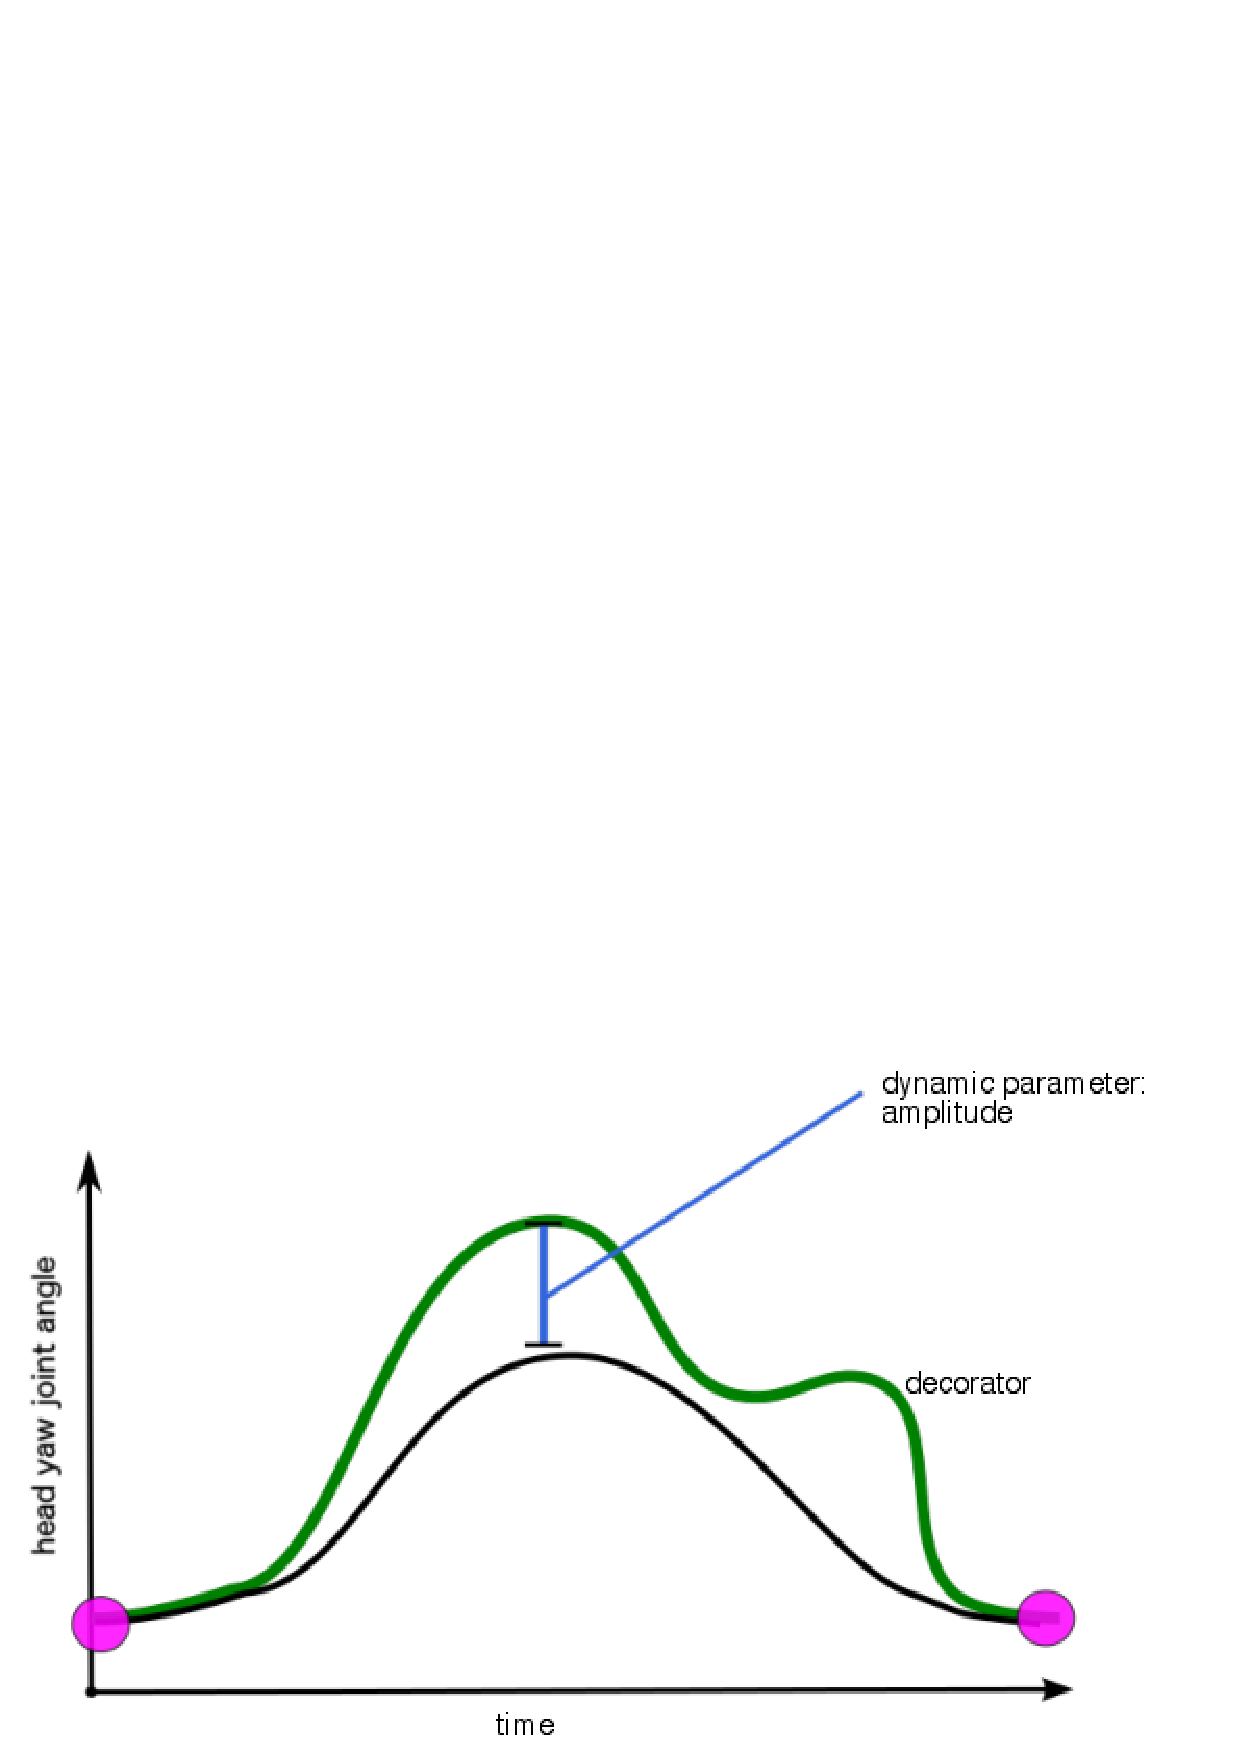
\includegraphics[width=0.8\linewidth]{style_graph}
	\caption{Style parameters for Head Yaw(green is stylized motion, black is original, the P0 pose is in pink)}
	\label{fig:styles_parameters}
\end{figure}
%todo show more than 1 style and show noise
Figure \ref{fig:styles_parameters} shows an example of stylisation of a head yaw joint angle motion.
In this example, the static parameters are included in the $p0$ position.
The amplitude change is a part of the dynamic parameter. 
Finally the decorator is an additional keyframe with a new value. 
The decorator is often an additional motion that is fused with the current motion.

\paragraph{Static parameters} allow to describe the neutral pose \texttt{p0}. 
This neutral pose \texttt{p0} is the posture the robot will take by default.
Sometimes, some joints of the body won't be in motion,  and hence the robot will keep the joint values of \texttt{p0}.
As before, we define this pose in accordance with the styles found in the literature. 
There are several static parameters that exist to describe poses. 
\texttt{p0} is very platform dependent. 

The definition of the pose is made in a specific file for each robotic platform. 
The style modeller makes a reference to this file in order to build the stylized motion at runtime and adds p0 before and after each motion event to ensure that it is the default pose.




\paragraph{Dynamic parameters}
From the literature in HRI and virtual agents in the domains of animation and psychology, we have listed some dynamic parameters that can be useful to depict changes in styled motion.
The current implementation of styles take into account the following parameters. 
%todo put a bit more detail in how it works
\begin{itemize}[noitemsep,nolistsep]
	\item Amplitude: the spacial extent related to the dimension of expansiveness from Gallaher and Meharbian.
	\item Speed: temporal extent and the velocity of execution of the movement.
	\item Tempo: specifies a rhythm for the key-frames in the motion (that are spaced according to the tempo).
	\item Noise: opposed to fluidity, noise makes the movements jerky where smoothing makes the movement fluid.
\end{itemize}
These parameters are set for each style, and for each of them, an algorithm takes the current motion and the value of this dynamic parameter to compute a new motion.
For instance, one can double the amplitude, change the tempo to 10Hz, add noise to the motion or slow down the motion.

\section{Model Validation}
Prior to this experiment, a first online study was performed. 
This online study aimed to ensure that generated styles were perceptible by end-users. 
93 parents watched videos of robots with 2 styles. 
We 


\section{Research Questions and Scenario}\label{sec:research-questions-and-scenario}
After the on-line study, this experiment aimed to do a real user experiment in an ecological environment in order to test the credibility and the acceptability of styles by children. 

One of the research questions behind the experiment was to test the style model and the plasticity model of the companion proposed. 

In this experiment, the same styles - Authoritative and Permissive -  as the ones were applied to the robots were used.
From these previous results, Authoritative and Permissive styles seemed to be identifiable by parents and applicable to the Nao robot \cite{Johal2014}. 

With this experiment, we wanted to verify our plasticity framework applied to HRI in a more general manner. 
In that sense, this experiment was also questioning versatile vs specialist robots. 
The aim here was to collect opinions of parents and children on the versatility of a companion robot and see if it was preferable to have a companion robot able to play several roles or does it affect its credibility and trust in accomplishing the tasks to be versatile.

In the experiment scenario, the child alone at home has to review his multiplication tables. 
His Teacher companion is here to ask him questions and to check if he knows them. 
After some questions, the companion(s) propose to dance for the child (faking that it has a dance competition) taking the Buddy role. 
However, some more questions of the math quiz have to be answered by the child and the companion retakes the Teacher role.


Following are a list of our principal hypothesis :
\begin{itemize}[noitemsep,nolistsep]
	\item[H0] Authoritative robots are perceived to be more dominant than permissive by children.
	\item[H1] Styles influence children's engagement in an interactive task.
	\item[H2] Styles influence the perceived competence and credibility of the robot in an interactive task.
	\item[H3] Styles influence the complicity with the robot in an interactive task.
	%\item[H4] Versatility of a companion increases the attachment and engagement of the children in interaction with it.
	\item[H4] Role-Specialist robots are perceived to be more competent and trustworthy than versatile robots.
	%\item[H6] There is an influence of the style during the math quiz during the dance on the child's behaviour.
\end{itemize}
%todo sentence for expe
Within subjects with put the conditions
\subsection{Subjects/Participants}
16 children and their their relatives participated to the experiment. 
Most often, the relatives were parents, but 3 children came with their grand-parents.
16 children participated to the experiment with ages from  
%todo boy and girl, and age and sd of age

\subsection{Apparatus/Materials}
The experiment took place in an ecological environment at Domus.
\footnote{Domus is an experimental platform of the LIG Laboratory.
	It contains a fully equipped and functional apartment with a kitchen, an office/living-room (where the experiment took place) and  a bedroom (where the interviews of the children took place)
	A sound and video direction room, from where the parents and another experimenter accessed audio and video capture in the apartment and record from the control PCs}
We added a Kinect sensor and a wooden board on the floor to avoid the robot falling. 
The Domus apartment is controllable by the OpenHab\footnote{\url{http://www.openhab.org}} middle-ware. 
OpenHab is a home control middle-ware that supports various sensors, protocols and operating systems. 
We were able, for instance, to launch music playback on the speaker of the apartment directly form the robot, by doing a simple HTTP\_REQUEST. 

Each interaction with the Nao robot(s) lasted about 15 minutes. 
Every child passed two sessions. 
For every child, we had about 30 minutes of recording of the interaction itself (a bit more because we also recorded explanations of the experimentalist). 
Every session was about 250Gb of recorded data on the disk. 
In total, we have collected about 8To of data. 


\section{Measures}
\subsection{Self-Assessment Measures}
The parents and the children are interviewed to collect data on acceptability, trust and  credibility of all the robots' performances and behaviors after each session. 
This evaluation allows us to do a comparison between conditions and between parents and children.

In order to collect the parents' and children's opinions on the interaction, we conducted interviews after each session.
These interviews aimed to collect the parents' and children's perception of the robot.
Building an interview that would suit both parents and children was a hard task\footnote{Interviews and Questionnaire used are available online: }.%todo put online

The first part of the interview is composed of very generic questions about the experiment. 
We then have more specific questions, and we finish by opening to other context of use of the robots.
The last questionnaire used after the second session is based on the Godspeed\cite{Bartneck2008b} items about Credibility, Likeability and Complicity. 
We also used the COIRS~\cite{Robert2014} questionnaire and adapted it for the parents.
After each session, the parents and the children would reply to the interview; and after the second a final interview would deal with explicit comparison of the two sessions by the participants.

\subsection{Quantitative Measures}
In addition to these qualitative evaluations at the end of the last session, the participants are asked to reply to a final survey in which they compare the conditions directly. 
This allows us to obtain the participants' preferences and to see if it is correlated to other measures. 
Objective measures are also collected to evaluate variations in the performance of children at the math test, and the engagement in the different tasks using the Kinect Sensor.

The engagement analysis is computed from skeleton data.
We base our quantitative analysis body measures defined in the Psychology literature.
This analysis will allow us to compare behaviour of the child according to the robot's style in front of him and to the versatility of the robot.

%\subsection{Data capture}
%\begin{figure}[h]
%	\begin{tabular}{|c | c|}
%		\hline
%		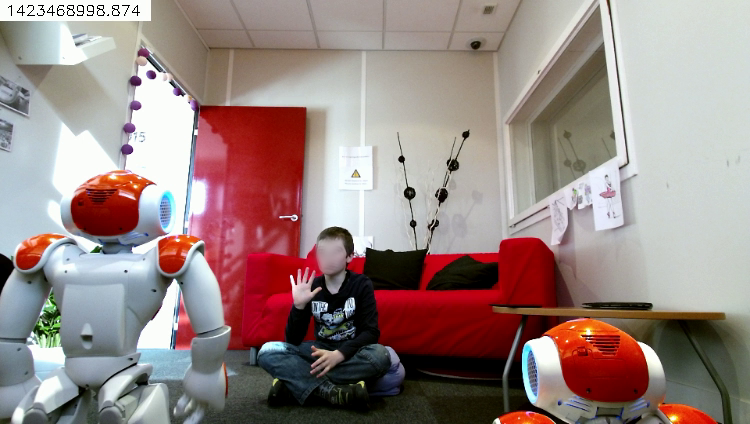
\includegraphics[width=0.45\linewidth]{../Figures/illustrate/k2a}&
%		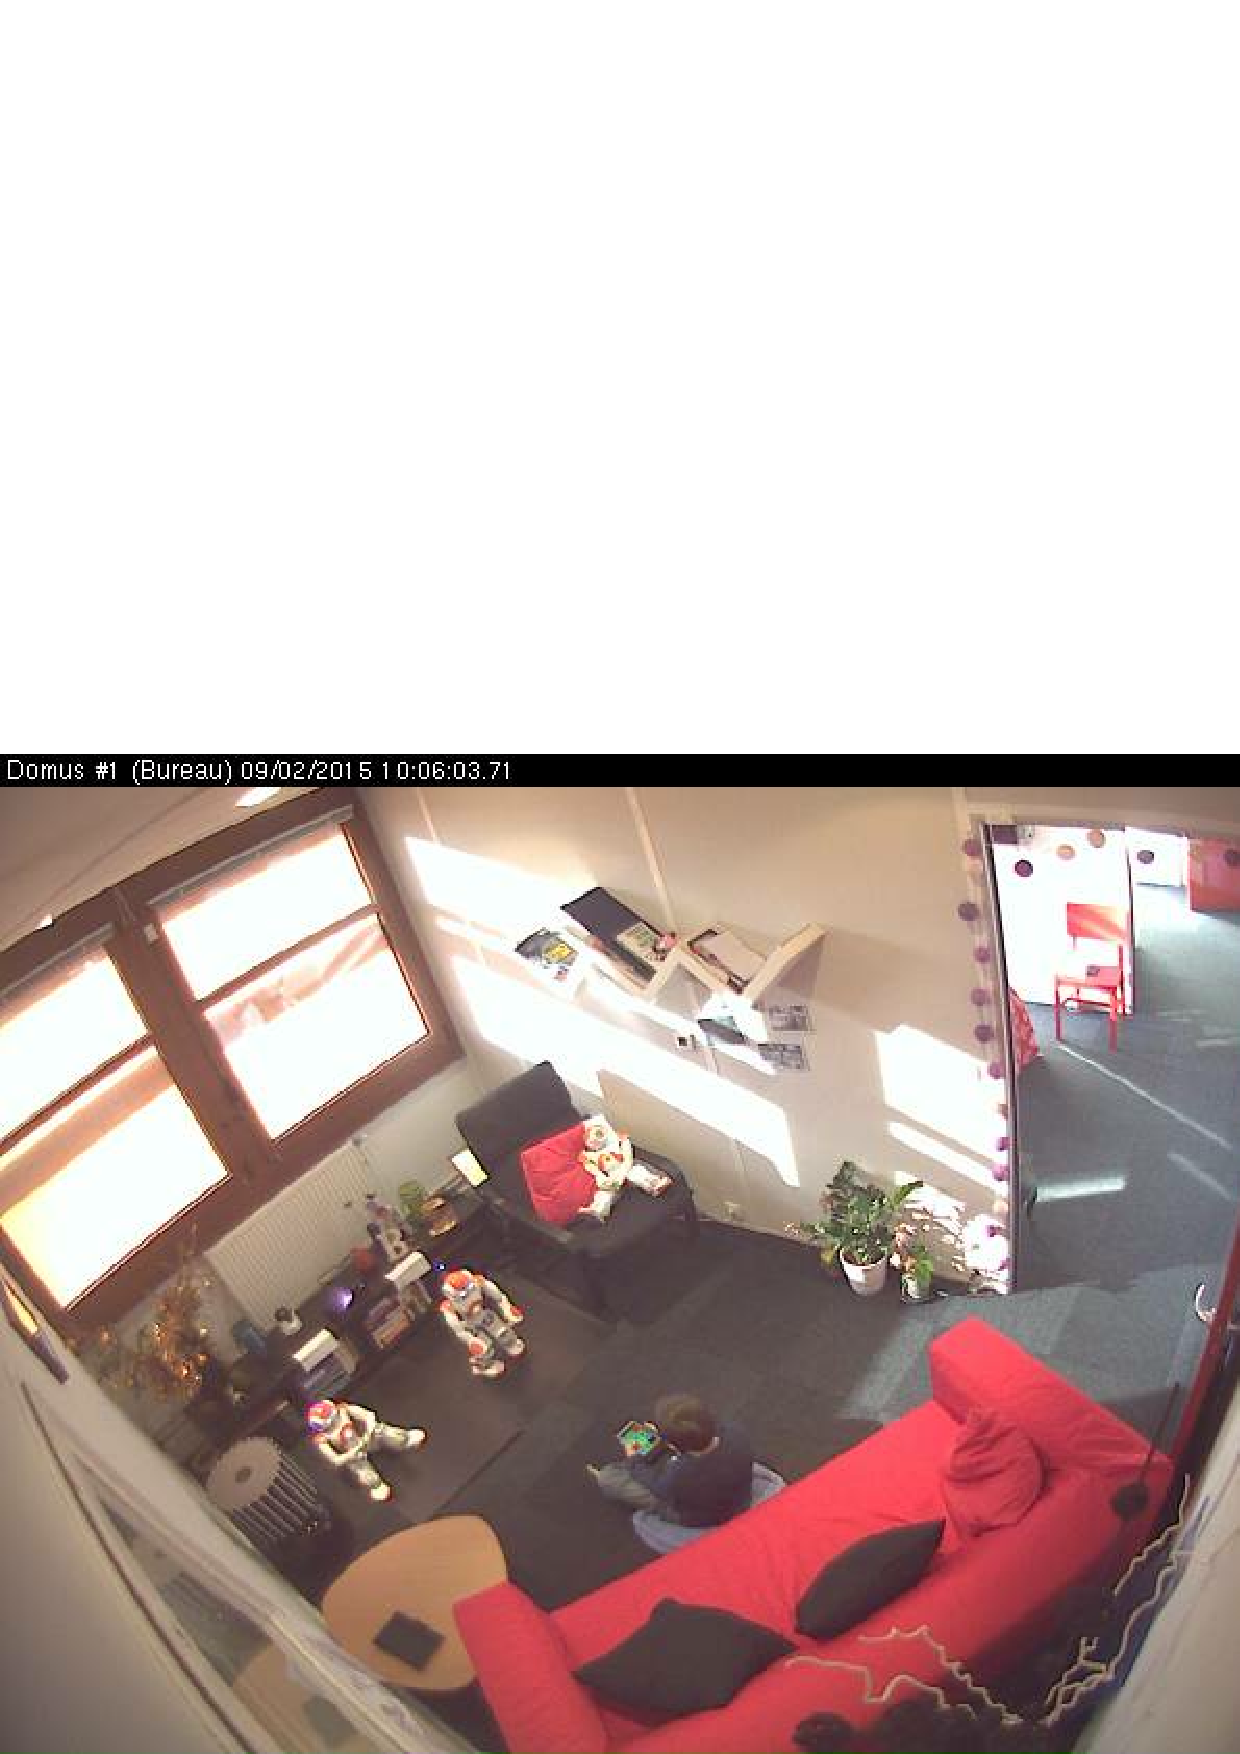
\includegraphics[width=0.45\linewidth]{ceilingb1}\\
%		Image from video capture from Kinect View &
%		Ceiling Back View \\\hline
%		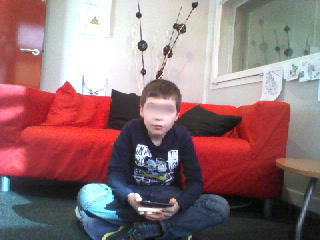
\includegraphics[width=0.45\linewidth]{./robotview}&
%		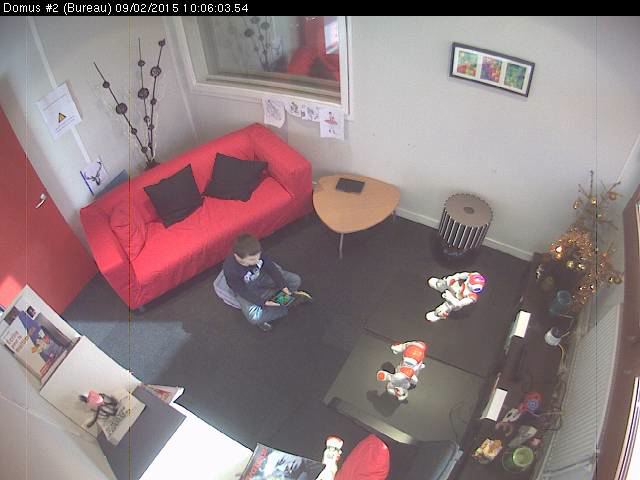
\includegraphics[width=0.45\linewidth]{ceilingf1}\\
%		Robot's Camera View &
%		Ceiling Front View\\ \hline
%	\end{tabular}
%	\caption{Samples of Video captures from the 4 cameras in the experiment}
%	\label{fig:allcam}
%\end{figure}

In order to be able to analyse the impact of the robot's style on the child's behaviour, we used a Kinect sensor and recorded all the available channels. 
It was a Kinect Sensor 2 from Microsoft. 

We used a program developed for MobileRGB-D to record raw data from the Kinect at a frame rate of 30FPS~\cite{MobileRGB}. 
Two video cameras in the ceiling (Fig. \ref{fig:allcam})  were also recording the interaction and were allowing the parents to see the interaction live in the control room. 
The robot was recording logs of the interaction with the tablet (question, answers and timestamps) that were after used to label the activities  automatically.  
We also recorded videos from the robots' cameras. 
For one of the children, a GoPro camera was also used to have images of the child's point of view during the interaction (Fig. \ref{fig:gopro2}).




The recorded data is summarised in table \ref{tab:dataset}
\begin{table}[h]
	\centering
	\caption{Data recorded during the interaction with the robots}
	\begin{tabular}{l p{1cm} p{1.5cm} p{2.5cm}}
		\hline
		Data  & Sensor & Frequency & \\ \hline
		RGB Video & Microsoft Kinect 2 & 30 Hz max & Resolution 1900*1080p \\
		Depth & Microsoft Kinect 2 & 30 Hz max & Resolution 512*424p from 40cm to 4.5m \\
		Body & Microsoft Kinect 2 & 30 Hz max & 6 bodies maximum with 25 joints (3D positions and 3D orientations as quaternions)\\
		Infrared & Microsoft Kinect 2 & 30 Hz & Resolution 512*424p \\ 
		Audio & Microsoft Kinect 2 &  &  \\
		\hline
		Video & Ceiling Office 1 & less than 30 Hz & Resolution 640*480 \\
		Video & Ceiling Office 2 & less than 30 Hz & Resolution 640*480 \\
		\hline
		Video & Nao Robot 1 & 15 Hz & Resolution 320*480 \\
		Video & Nao Robot 2 & 15 Hz & Resolution 320*480 \\
		\hline
	\end{tabular}
	\label{tab:dataset}
\end{table}


Each session lasted about 15 minutes. 
Every child passed two sessions. 
For every child, we had about 30 minutes of recording of the interaction itself (a bit more because we also recorded explanations of the experimentalist). 
Every session was about 250Gb of recorded data on the disk. 
In total, we have collected about 8To of data. 

%\subsection{Samples of recorded data}
%todo maybe add samples






\subsection{Measures Extracted from Body Analysis}
We used the skeleton data to measure variation on the child's attitude between the sessions.
Several features form the literature of body communication have been implemented and applied for the Body Kinect data.


\paragraph{Torso and Neck Orientations}
TorsoQ and NeckQ are given by the Kinect sensor to be respectively the mid-spine joint and the neck orientations. 
These features are formalised as in the form of quaternions. 
In order to illustrate  these angles clearly, we converted the quaternions to euclidean angles in the graphs.
Figure \ref{fig:neckrelax} shows the neck relaxation angle.

\paragraph{Leaning angle}
Leaning left and right corresponds sideways lean (see Fig. \ref{fig:sideways_lean}), while leaning forward and back corresponds to frontal leaning angle (see Fig. \ref{fig:BLA}). 
The values range between $-1$ and $1$ in both directions, where 1 roughly corresponds to $45\deg$ of lean.

In addition to the given angles from the Kinect sensor for the leaning angles, we computed a body lean angle in line with the work of \cite{Castellano} and \cite{Schegloff}. This angle, was computed by the dot product of the vertical vector from the hip centre joint and the vector from the hip centre to the shoulder centre of each collected body data frame. 

\paragraph{Volume}
For each frame, the volume is computed by going through the joints and recording the min and max in all three dimensions (X,Y,Z). 
We also use as feature the joint's name at the minimum and the maximum for all three dimensions.

\paragraph{Status of Hands}
The status of hands IS given by the Kinect Sensor with values ranging among Open, Closed, Lasso, NotTracked and Unknown. 
This feature is considered to be a good candidate for Hand Relaxation, advocated by Meharbian~\cite{Meharbian} as a sign of relaxation. 
Only the Open and Closed recognition are exploited. 


\paragraph{Asymmetry Values}
According to \cite{Mehrabian}, a high degree of asymmetry in arms and legs are cues to looseness and the relaxation of the body.
In order to compute the asymmetrical rate of the members, we computed the dot products of vectors for the joints(see Figure \ref{fig:arm_asymmetry2}). 

%\paragraph{Rocking Movements (0.91)}: number of times S changes his angle of forward-back lean of torso by 10 deg or more. Again









\section{Results}
%Statistics
%ANOVA results are cited using the F test (e.g., $F (1, 38) = 4.94$, $p = .04$). F and p are italicized. Give the exact $p$ value to two decimal places except when greater better than $p < .01$. Try to avoid more than two decimal places, as readers are not very interested in exact values; comparisons are more important. The $F$ value is followed by the degrees of freedom in the numerator and denominator. Here is how one author of a mobile phone study (Author, 2010) reported an interaction effect:
%\begin{quotation}
%The data were analyzed in a 2 (Age: young vs. old) x 2 (Device: Phone A vs. B) mixed measures analysis of variance (ANOVA). We found an interaction of Age X Phone ($F [1, 38] = 26.18$, $p < .0001$). The contrast showed older people using Phone B took considerably longer to complete the task, $F (1, 38) = 69.16$, $p = .02.$ (p. 6).
%\end{quotation}
%Correlations using product moment tests are reported using $r$ (e.g., $r (200) = .19$). The number in parenthesis following the $r$ value represents the degrees of freedom ({\it df}),  or N Ð 1. Including the degrees of freedom provides the reader with a sense of statistical significance, in that correlations are highly sensitive to the number of data points. For instance, with 200 scores on both variables, .19 will be a significant correlation whereas with only 30 people, it will not be statistically significant.
%
%T tests (e.g., $t [20] = 100.2$, $p < .01$) are reported giving the degrees of freedom in the denominator. (The numerator {\it df} is always $1$, as is true of correlations.)
%Notice how brackets are placed inside parentheses to reduce confusion.



\section{Discussion}
\section{Conclusion}
%original hypothesis:
The need for social customization of companion's robot behaviour led us to propose behavioural styles and to assume that it was possible for users to distinguish between styles and, and that they were impacting the robot-user interaction.

%Findings
The \dots model provided realistic simulations of \dots for these two \dots and may be applicable to other types of \dots.

%Explanation for findings


%Limitations
However, the model contains 

%Need for further research


%futur for styles and personalisation
In the future, even the appearance should be customizable by the user since some studies have shown that there exist systematic individual differences in terms of preference of the companion's appearance \cite{Walters2008}. 
They have highlighted individual differences in the preference of the robot's dynamic which could suggest and emphasise the need for the social adaptation of robots. 
From these researches the Uncanny Valley\footnote{Uncanny Valley:} is not at the same location for each individual and the creepiness threshold might also be varying. 




%*****************************************************************************************************


%*****************************************************************************************************


%
%\section{Table of Behaviours for each style factor from \cite{Gallaher1992}}
%\label{tab:styledims_gallaher}
%\begin{table}[h]
%	\small
%	\centering
%	\begin{tabular}{|l |c|  l |}\hline
%		\textbf{Behavioural Items}  &	\textbf{Style factor} & Computationable term \\ \hline
%		Uses very little-most of body when gesturing & Expressiveness  & TODO \\
%		Slow-fast gestures  & Expressiveness & Velocity \\
%		Gestures: infrequently-frequently & Expressiveness & QOM\\
%		Shakes head: frequently-rarely & Expressiveness &  head motion and head angular velocity in 3D\\
%		Narrow-broad gestures & Expressiveness & Extensiveness \\
%		Nods head: frequently-rarely & Expressiveness & head motion and head angular velocity in 3D \\ \hline
%		
%		Shoulders: slumped-erect when standing & Animation & shoulder opening angle\\
%		Sits down and stands up: slowly-quickly & Animation & TODO\\
%		Torso: upright-leaning when standing & Animation & torso lean angle\\
%		Sits with torso: tilted-vertical & Animation & todo\\
%		Slow-fast walker & Animation & none\\
%		Sits with torso: erect-slumped & Animation & todo? \\ \hline
%		
%		Legs: together-wide apart when sitting & Expansiveness & legs extensivess\\
%		Soft-loud voice & Expansiveness\\
%		Elbows: close to-away from body & Expansiveness & elbows distace to core\\
%		Thin-full voice & Expansiveness\\
%		Light-heavy step & Expansiveness\\
%		Takes: small-large steps & Expansiveness\\
%		Legs: close together-wide apart when standing  & Expansiveness\\
%		Hands: close to-away from body & Expansiveness \\ 
%		Soft-loud laughter & Expansiveness\\ \hline
%		
%		Choppy-rhythmic speech & Coordination\\
%		Jerky-fluid walk & Coordination & jerkiness\\
%		Rough-smooth gestures & Coordination\\
%		Harsh-smooth voice & Coordination\\ \hline
%		
%	\end{tabular}
	%\caption{Table of Behaviours for each style factor from \cite{Gallaher1992}}
	
%\end{table} 




\section{Acknowledgements}
This work is conducted within a project aiming to design a world of artificial companions, the French funded ANR My Little World of Artificial Companions - MOCA project, ANR-2012-CORD-019-02.

\small
\bibliographystyle{abbrv}
\bibliography{jsoro16.bib}


\end{document}
